\documentclass[11pt,a4paper]{article}

\usepackage[utf8]{inputenc}
\usepackage[T1]{fontenc}
\usepackage{geometry}
\usepackage{titlesec}
\usepackage{graphicx}
\usepackage{float}
\usepackage{xcolor}
\usepackage{listings}
\usepackage{hyperref}
\usepackage{enumitem}

\geometry{margin=2.5cm}

\hypersetup{
    colorlinks=true,
    linkcolor=blue,
    urlcolor=blue
}

\titleformat{\section}
{\large\bfseries}
{\thesection.}{0.5em}{}

\titleformat{\subsection}
{\normalsize\bfseries}
{\thesubsection.}{0.5em}{}

\definecolor{codebg}{rgb}{0.95,0.95,0.95}

\lstset{
    backgroundcolor=\color{codebg},
    basicstyle=\ttfamily\small,
    frame=single,
    breaklines=true,
    columns=fullflexible
}

\begin{document}

\begin{titlepage}
    \centering

    \vspace*{3cm}

    {\Huge \textbf{SSH Hardening and Intrusion Prevention}}\\[1cm]

    {\Large Server Engineering Labs}\\[2cm]

    \textbf{Author:}\\
    Laura Ortiz Moreno\\[1cm]

    \textbf{Topics Covered:}
    \begin{itemize}[leftmargin=4cm]
        \item SSH server configuration
        \item Key-based authentication
        \item Port hardening
        \item Firewall management
        \item Fail2ban intrusion prevention
        \item Secure remote administration
    \end{itemize}

    \vfill

    \textbf{Environment:}\\
    Debian Linux Virtual Machine\\
    Rocky Linux Client VM\\
    Virtualized lab environment

    \vspace{1cm}

\end{titlepage}

\tableofcontents
\newpage

\section{Introduction}

This report documents the configuration and hardening of SSH services in a Linux server environment.

The goal of the laboratory was to:
\begin{itemize}
    \item Configure secure remote access
    \item Replace password authentication with SSH keys
    \item Reduce exposure to automated attacks
    \item Configure firewall rules
    \item Deploy Fail2ban for intrusion prevention
\end{itemize}

The exercises were performed in a client-server virtualized environment using Debian and Rocky Linux virtual machines.

\section{SSH Service Verification}

The first step consisted of verifying that the SSH service was installed and active.

Useful commands included:

\begin{lstlisting}[language=bash]
sudo systemctl status ssh
sudo ss -tulpn
\end{lstlisting}

These commands allow administrators to:
\begin{itemize}
    \item Check whether the SSH daemon is running
    \item Verify listening ports
    \item Inspect active network services
\end{itemize}

\section{Changing the Default SSH Port}

To reduce exposure to automated scans and brute-force attacks, the default SSH port was modified.

The SSH configuration file was edited:

\begin{lstlisting}[language=bash]
sudo nano /etc/ssh/sshd_config
\end{lstlisting}

The default port:

\begin{lstlisting}
Port 22
\end{lstlisting}

was replaced with a custom port:

\begin{lstlisting}
Port 22022
\end{lstlisting}

\begin{figure}[H]
    \centering
    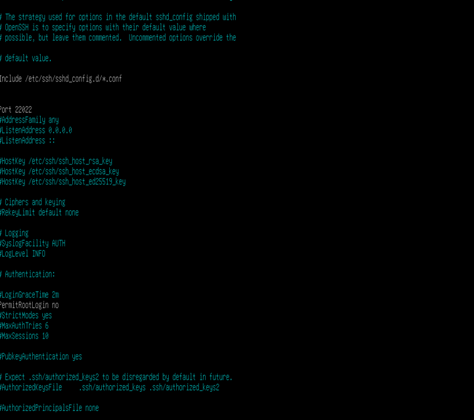
\includegraphics[width=0.88\textwidth]{images/ssh/sshd-config.png}
    \caption{Customized SSH daemon configuration using a non-default port and hardened authentication settings.}
\end{figure}

The SSH service was then restarted:

\begin{lstlisting}[language=bash]
sudo systemctl restart ssh
\end{lstlisting}

\subsection{Firewall Configuration}

Firewall rules were updated to allow connections through the new port.

Example using UFW:

\begin{lstlisting}[language=bash]
sudo ufw allow 22022/tcp
sudo ufw reload
\end{lstlisting}

\section{SSH Key Authentication}

Key-based authentication was configured to improve security and avoid password-based login.

SSH keys were generated on the client machine:

\begin{lstlisting}[language=bash]
ssh-keygen -t ed25519
\end{lstlisting}

The public key was copied to the server:

\begin{lstlisting}[language=bash]
ssh-copy-id -p 22022 user@server
\end{lstlisting}

A successful login test was then performed:

\begin{lstlisting}[language=bash]
ssh -p 22022 user@server
\end{lstlisting}

\begin{figure}[H]
    \centering
    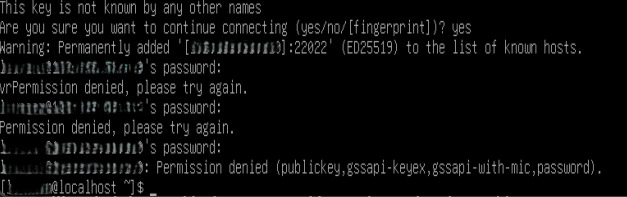
\includegraphics[width=0.90\textwidth]{images/ssh/ssh-failed-login-test.png}
    \caption{SSH authentication test performed against the hardened SSH service using the custom port configuration.}
\end{figure}

\subsection{Security Considerations}

Benefits of SSH keys include:
\begin{itemize}
    \item Stronger authentication
    \item Protection against password brute-force attacks
    \item Easier automation of administrative tasks
\end{itemize}

\section{Disabling Password Authentication}

After verifying that key authentication worked correctly, password authentication was disabled.

The following parameters were modified in:

\begin{lstlisting}
/etc/ssh/sshd_config
\end{lstlisting}

\begin{lstlisting}
PasswordAuthentication no
PermitRootLogin no
\end{lstlisting}

The service was restarted afterward:

\begin{lstlisting}[language=bash]
sudo systemctl restart ssh
\end{lstlisting}

\section{Fail2ban Installation and Configuration}

Fail2ban was installed to automatically block repeated failed login attempts.

Installation:

\begin{lstlisting}[language=bash]
sudo apt install fail2ban
\end{lstlisting}

The service status was verified:

\begin{lstlisting}[language=bash]
sudo systemctl status fail2ban
\end{lstlisting}

\subsection{SSH Jail Configuration}

A local configuration file was created:

\begin{lstlisting}[language=bash]
sudo nano /etc/fail2ban/jail.local
\end{lstlisting}

Example configuration:

\begin{lstlisting}
[sshd]
enabled = true
port = 22022
maxretry = 5
bantime = 10m
findtime = 10m
\end{lstlisting}

\subsection{Monitoring Banned Attempts}

Fail2ban status commands:

\begin{lstlisting}[language=bash]
sudo fail2ban-client status
sudo fail2ban-client status sshd
\end{lstlisting}

\begin{figure}[H]
    \centering
    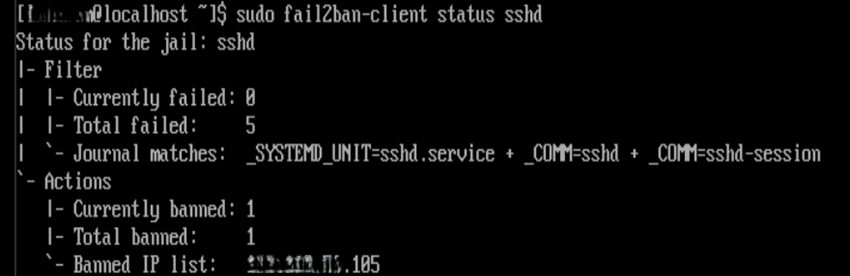
\includegraphics[width=0.90\textwidth]{images/ssh/fail2ban-ban-status.png}
    \caption{Fail2ban jail status showing detection and automatic banning of repeated failed SSH login attempts.}
\end{figure}

\begin{figure}[H]
    \centering
    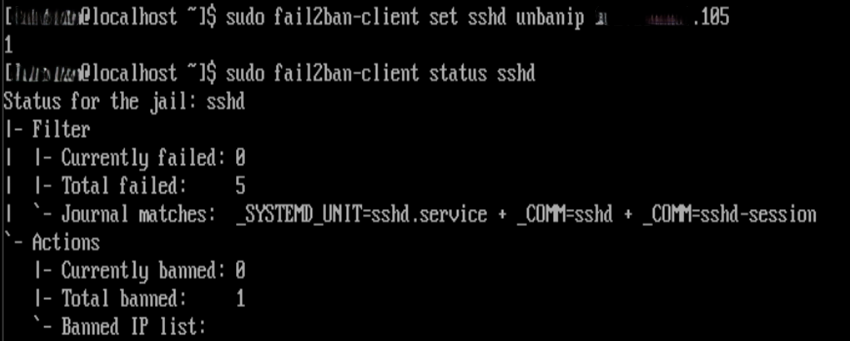
\includegraphics[width=0.90\textwidth]{images/ssh/fail2ban-unban-status.png}
    \caption{Manual unban operation and updated Fail2ban SSH jail status after removing the blocked client.}
\end{figure}

\section{Remote Access Validation}

Several validation tests were performed:
\begin{itemize}
    \item SSH login through the custom port
    \item Key-only authentication
    \item Verification of blocked failed attempts
    \item Firewall validation
\end{itemize}

The hardened configuration successfully reduced exposure while maintaining remote administration functionality.

\section{Challenges Encountered}

Several configuration issues appeared during the lab:
\begin{itemize}
    \item Incorrect firewall rules blocking SSH access
    \item SSH restart failures due to configuration syntax errors
    \item Key permission problems
    \item Fail2ban misconfiguration during testing
\end{itemize}

Special care was required because incorrect SSH settings may completely block remote access to the server.

\section{Conclusion}

This laboratory provided practical experience in Linux server hardening and secure remote administration.

The exercises demonstrated:
\begin{itemize}
    \item SSH configuration and troubleshooting
    \item Secure authentication using SSH keys
    \item Firewall configuration
    \item Basic intrusion prevention with Fail2ban
    \item Security-oriented system administration practices
\end{itemize}

These concepts are fundamental in Linux infrastructure administration, cybersecurity, and production server environments.

\end{document}